\chapter{Literature Review}

\label{literature_review}

\section{Pellet-cladding interaction (PCI)}

When a fuel pin is first inpile, there is a gap between the fuel pellet and the cladding (see § \ref{ss_fuelpin}). This gas gap slowly closes over time, mostly due to thermal expansion and swelling of the fuel pellet (illustrated in Figure \ref{figure:pcmi}) due to radiation damage and the accumulation of fission products. At a high enough burnup, the fuel pellet finally makes contact with the cladding. This phenomenon is called pellet-cladding interaction (PCI) and involves both mechanical and chemical interactions which contribute to observed fuel failures.

\begin{figure}[ht] % PCMI bambooing
\centering
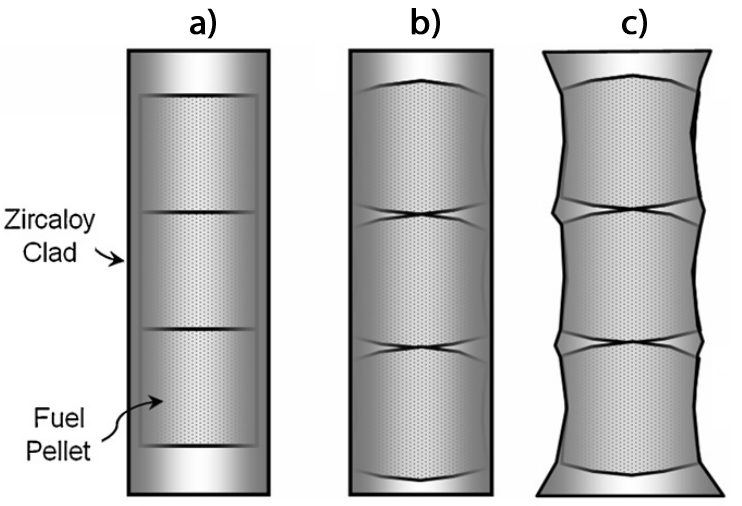
\includegraphics[width=13cm]{images/pcmi.png}
\caption[Illustration of fuel swelling and clad deformation due to PCI. \textbf{a)} Fresh fuel before irradiation. \textbf{b)} Thermal expansion and swelling of fuel pellets and closing of fuel-pellet gap during operation. \textbf{c)} Fuel contact with cladding and subsequent `bambooing' of the cladding.]{Illustration of fuel swelling and clad deformation due to PCI. \textbf{a)} Fresh fuel before irradiation. \textbf{b)} Thermal expansion and swelling of fuel pellets and closing of fuel-pellet gap during operation. \textbf{c)} Fuel contact with cladding and subsequent `bambooing' of the cladding. Adapted from \cite{alam2011review}.}
\label{figure:pcmi}
\end{figure}

PCI-related failure of nuclear fuel pins has been known about since 1963, when the first reported failure occurred in a highly rated fuel pin during reactor start-up \cite{lyons1963high}. Many studies have since been made regarding the topic \cite{alam2011review, bcoxpelletclad1990}. The exact cause of PCI failures has not yet been determined, however it is likely that both the mechanical and chemical effects of contact between the fuel pellet and the cladding are necessary for it to occur. It is also known that PCI failures are typically preceded by power transients, such as during reactor startup where several power ramps are performed over many hours.

\subsection{Fuel pellet relocation}

Irradiated fuel pellets will sometimes crack and break into fragments while in the cladding. These fragments are unconstrained and are able to move radially outwards (i.e. towards the pellet-cladding gap). This phenomenon is called `relocation', although this term is also used to refer to movement of the pellet fragments in the axial direction within the cladding \cite{sheppard1982data}. Relocation of fuel fragments means that firm contact between the fuel and cladding can occur earlier in the fuel pin's life (i.e. before fuel swelling closes the fuel-cladding gap).

The conceptual model of fuel pellet relocation is shown in Figure \ref{figure:relocation} as a plot of the `effective' gap (based on cladding temperature and fuel centreline temperature) against rod power. Initially, the fuel pellet has no fragmentation and a wide fuel-cladding gap (region I). The gap decreases slowly due to thermal expansion as rod power is increased until point A where the fuel pellet cracks and fragments. The fuel pellet fragments move radially outward and the gap decreases significantly (region II). Point B marks the onset of `soft' PCI, meaning that the fuel pellet fragments make some contact with the cladding, but are not yet fully constrained (e.g. radial or azimuthal motion is still possible). The fragments' lack of mechanical constraints prevent a stress from being imparted to the cladding, thus the mechanical interaction is considered `soft' (region III). At point C, thermal expansion due to rod power is large enough that some pellet fragments become mechanically constrained, marking the onset of `hard' PCI (region IV). As discussed in § \ref{ss_fuelpin}, chipping of fuel pellets can cause debris to occupy the pellet-cladding gap, thereby reducing the rod power at which onset of hard PCI occurs.

\begin{figure}[ht] % Relocation
\centering
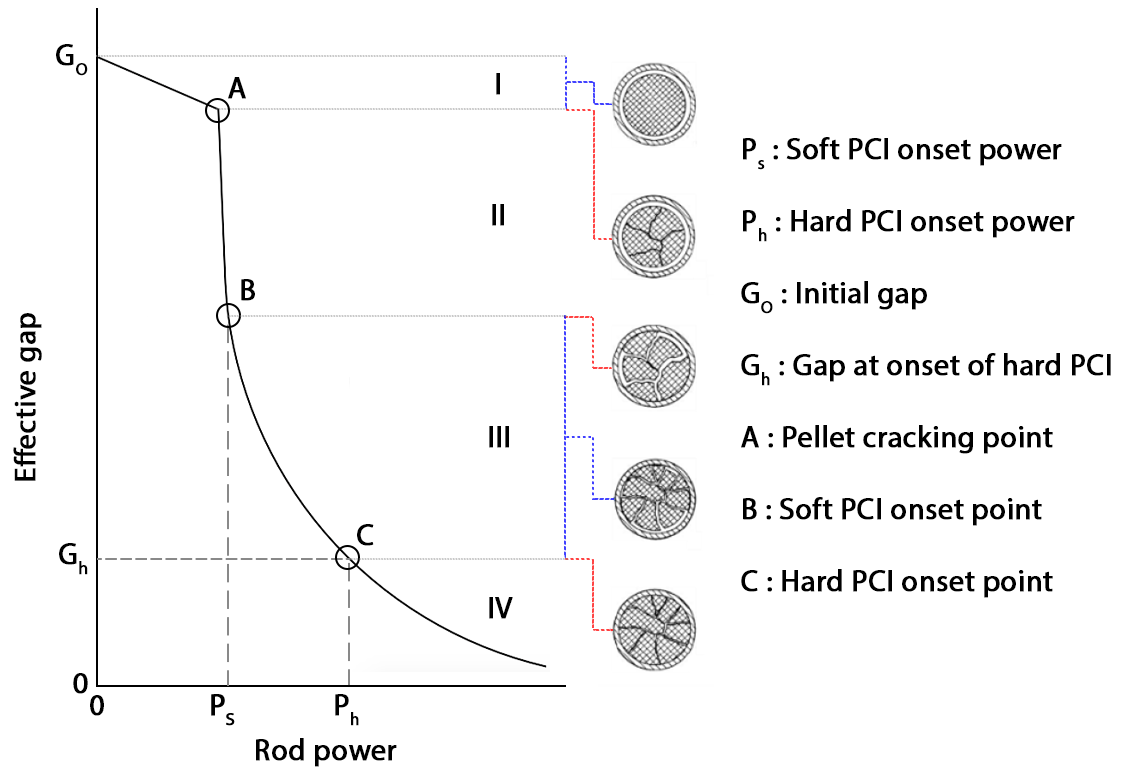
\includegraphics[width=15cm]{images/relocation.png}
\caption[Concept of pellet-cladding gap model showing stages of fuel pellet fragment relocation with onset of soft and hard PCI. ]{Concept of pellet-cladding gap model showing stages of fuel pellet fragment relocation with onset of soft and hard PCI. Adapted from \cite{Oguma1983} with fuel pin cross-sections from \cite{walton1983fuel}.}
\label{figure:relocation}
\end{figure}

\subsection{Pellet-clad gap and bonding}

The gap between the fuel and the cladding allows fuel pellets to be inserted into the fuel pin easily during manufacture, but this clearance is also designed to accommodate some increase in fuel pellet volume. It is important to consider the thermal expansion of the fuel pellet, as the centreline temperature of a PWR fuel pellet during a power transient can vary between 1500 and 1800 $^{\circ}$C, depending on the burnup of the fuel and magnitude of the reactivity insertion \cite{Bagger1994}. In addition, fuel pellets will swell due to radiation damage throughout their operational lifetime. Once the pellet-clad gap has closed entirely, any pellet expansion during a power transient will translate to a force exerted on the cladding, generating hoop stresses which open cracks on the inner cladding surface. This is the mechanical component of PCI.

When the fuel pellet makes contact with the cladding, there is also a chemical interaction between the UO$_{2}$ (and fission products) and the internal surface oxide of the cladding. UO$_{2}$ has some solid solubility in ZrO$_{2}$, and we therefore see a bonded reaction layer, which has a chemical composition (U, Zr)O$_{2}$.  Due to the large U atom, cation substitution allows this mixed layer to adopt the crystal structure of cubic fluorite, the high temperature phase of ZrO$_{2}$. The uranium nuclei in both this bonding layer and the outer rim of the fuel pellet experience the highest number of fission events (due to the proximity to the moderator), and therefore this region contains fission products that contribute to the chemical degradation of the fuel cladding, in particular iodine. This is the chemical component of PCI.

\subsection{Reactor power ramps}

It has been established that power ramping of the reactor is associated with PCI failures \cite{penn1977candu, MacDonald1979, Hardy1977198, Knaab1987}. This presents a problem for reactors when it comes to events such as start-up, load-following and any other power transients experienced by the fuel pins. Figure \ref{figure:reactor_startup} shows how reactor power varies over time during a typical PWR start-up procedure. A combination of low ramping rates and long holds at low power (to remain below ramping limits, to condition fuel \cite{billaux2005pellet}\footnote{Fuel is considered `conditioned' after it has operated at a specified power level for a certain period of time.}, and conduct coolant chemistry checks) require the entire procedure to be completed in a period of 90 hours, with several operator switch-overs in between. This is a costly procedure for the utility owner to perform, with millions of US\$ foregone in electricity sales for larger reactors.

\begin{figure}[ht]
\centering
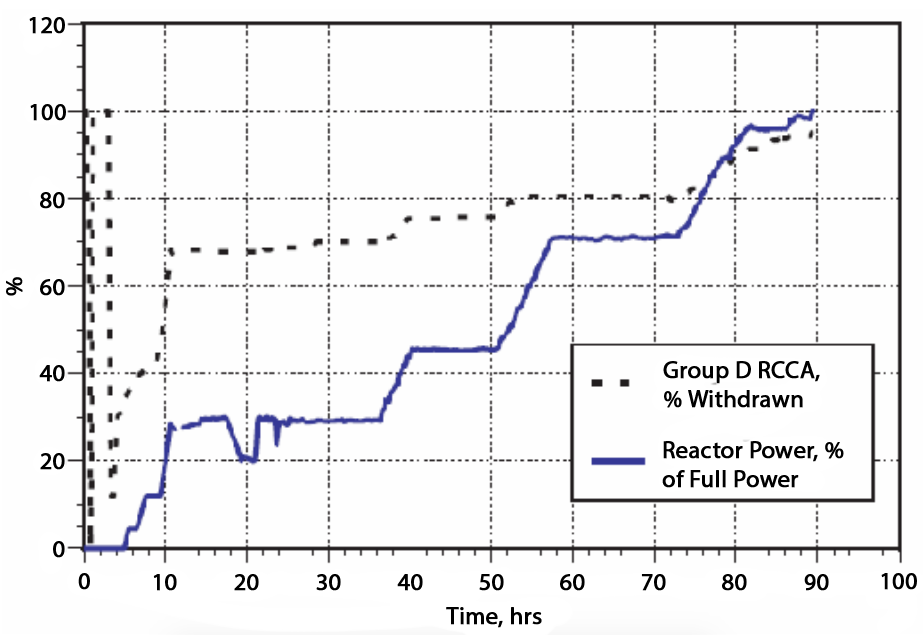
\includegraphics[height=10cm]{images/reactor_startup.png}
\caption[Reactor startup procedure for a typical US PWR. Dashed line indicates \% withdrawal of control rods.]{Reactor startup procedure for a typical US PWR. Dashed line indicates \% withdrawal of control rods. Adapted from \cite{ramping}.}
% M. F. James, R. W. Mills and D. R. Weaver (1991) UKAEA Reports, AEA-TRS-1015, AEA-TRS-1018 
         %  and AEA-TRS-1019.
\label{figure:reactor_startup}
\end{figure}

Scheduled reactor shutdowns or extended reduced power operation (ERPO) events occur whenever refuelling or maintenance of the reactor is required (and in some cases there may be a grid demand to reduce power output).  Refuelling is typically performed every 1 to 2 years, while maintenance may be required at any time. Emergency shutdowns may also occur and have their own challenges to consider (e.g. xenon poisoning, decay heat removal), though they are more rare. In each case, going through the lengthy power ramping procedure is required, and since these shutdowns cannot be avoided, being able to ramp up power faster would be a significant improvement. Ramp rates in reactors are restricted to between 3-4\% of full power per hour above a certain threshold level to avoid PCI failures \cite{ramping}. Additionally, fuel conditioning holds (operation at certain power levels for long periods) are performed to further reduce the incidence of PCI failures. 

These limits present a challenge not just when restarting reactors, but also for the implementation of load-following in reactors. PWRs have thermal feedback loops which provide some level of intrinsic load-following behaviour. For example, an increase in steam demand leads to increased boiling in the steam generators. The subsequent decrease in coolant temperature in the primary circuit leaving the steam generator causes a reactivity increase and therefore a power increase in the reactor. The reactor returns to critical (reactivity = 0) after some fluctuation, and the average temperature of the coolant remains unchanged.

\subsection{PCI Failures}

PCI failures are typically associated with cracks which span the thickness of the cladding (so-called \emph{pinhole} defects), subsequently causing fission product contamination of the primary loop coolant. A fuel cladding breach is detected when a sharp spike in radioactivity is registered by sensors in the primary loop (i.e. a signal that is distinguishable above the previous background). This means that the time to detection of a failure from the failure-inducing event (e.g. a power ramp) is known, but that the time taken for the PCI failure to occur is unknown \cite{bcoxpelletclad1990}. 

Figure \ref{figure:fuelcladdingcrack} shows the typical cracking behaviour of fuel pellets and cladding from a PWR fuel pin subjected to two annual operating cycles. % TODO

\begin{figure}[ht]
\centering
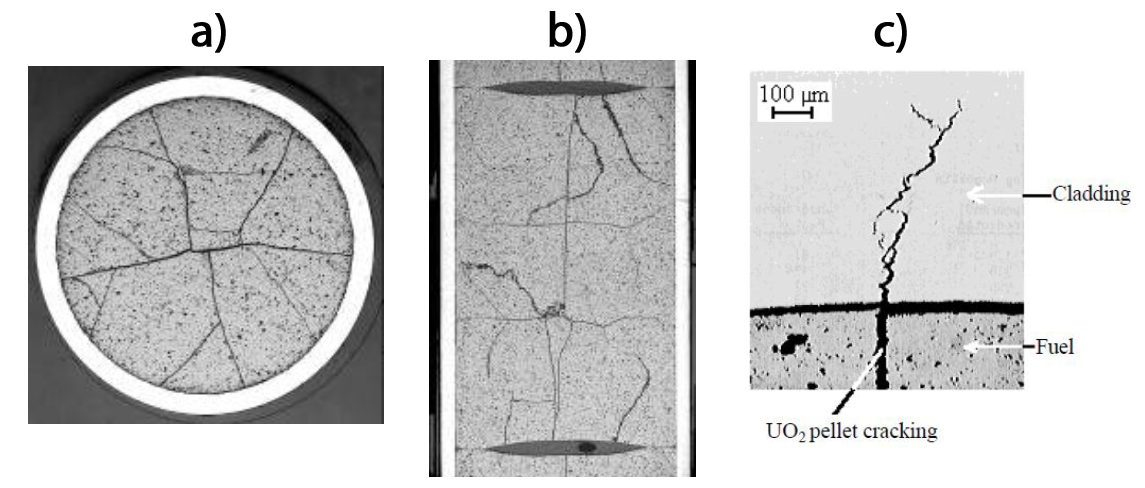
\includegraphics[width=\linewidth]{images/fuelcladdingcrack.png}
\caption[Cracking of PWR fuel pellets and cladding. \textbf{a)} Transversal macrography of a fuel rod irradiated for two annual PWR operating cycles. \textbf{b)} Axial macrography of a fuel rod irradiated for two annual PWR operating cycles. \textbf{c)} SCC cladding failure.]{Cracking of PWR fuel pellets and cladding. \textbf{a)} Transversal macrography of a fuel rod irradiated for two annual PWR operating cycles. \textbf{b)} Axial macrography of a fuel rod irradiated for two annual PWR operating cycles. \textbf{c)} SCC cladding failure. Adapted from \cite{brochard2001modelling}.}
\label{figure:fuelcladdingcrack}
\end{figure}

\subsection{Fission products and SCC}

Although PCI failures were found to occur during power ramping, it was not yet known whether these failures were due to fission product induced SCC or tensile failure of the cladding due to radiation embrittlement. 

In 1971, scientists at the Chalk River Nuclear Laboratories conducted a series of tests to determine if fission products were necessary \cite{MacDonald1979}. The experiments involved taking highly irradiated zirconium fuel pins (fluence of $8 \times 10^{24}$ n/m$^{2}$ with 1 MeV neutrons) and then inserting fresh, unirradiated UO$_{2}$ fuel pellets into them. These fuel pins were then inserted back into a reactor and subjected to large power ramps, as shown in Figure \ref{figure:fueltests}. These ramps (phase I and II) would typically cause failures in fuel pins with similar irradiation histories. In the initial ramp tests however, all the fuel pins survived the ramps intact. Six fuel pins were then irradiated in the reactor at low power to a burnup in excess of 50 MWh/kg U in order to build up fission products in the fuel (phase III). In a subsequent ramp test (phase IV), two of the high burnup fuel pins failed in the reactor. This finding provided the strongest evidence to date that fission products are necessary for PCI failure of zirconium-based claddings. The fission product most likely to cause cracking, based on known SCC susceptibility of Zr metal, is iodine.

\begin{landscape}
\begin{figure}[ht]
\centering
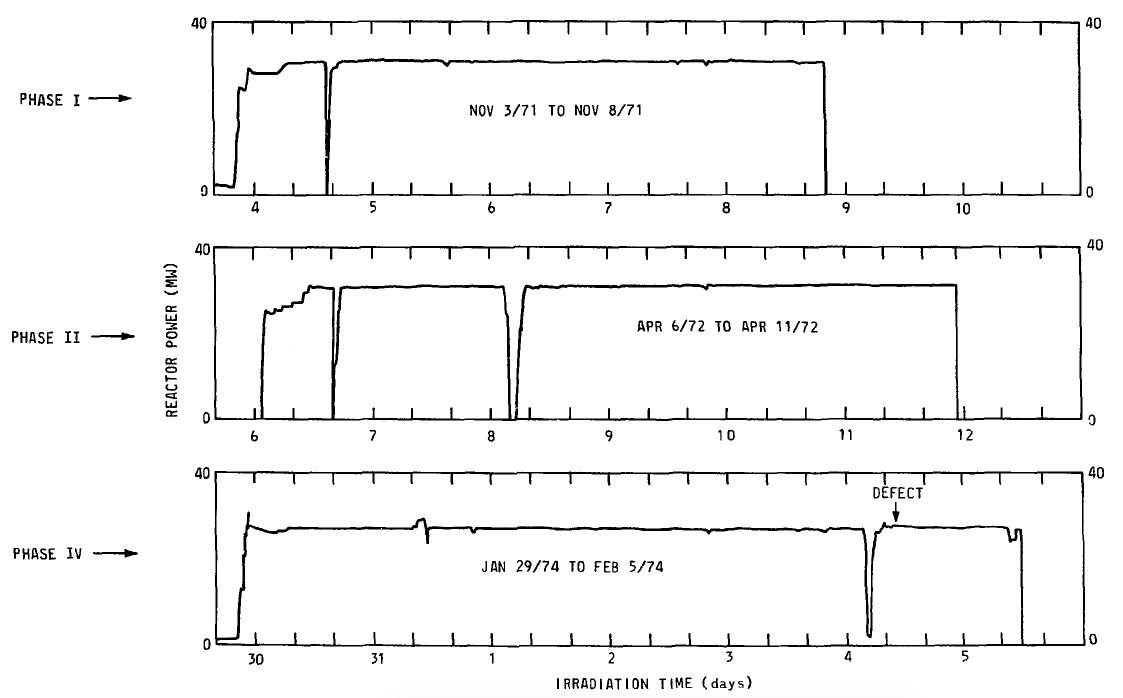
\includegraphics[width=\linewidth]{images/fueltests.png}
\caption[Power ramping test data for the different phases of the Chalk River Nuclear Lab experiment.]{Power ramping test data for the different phases of the Chalk River Nuclear Lab experiment. Taken from \cite{MacDonald1979}.}
\label{figure:fueltests}
\end{figure}
\end{landscape}

As discussed earlier, iodine is one of the most prevalent fission products and it is known to corrode zirconium metal \cite{iodinezrmetal, Sidky1998, rosenbaum1966interaction, Fregonese1998, Lewis2011, anghel2010experimental}. The exact mechanism by which this occurs in fuel pins is not yet known, though a combination of radiolysis, I$_{2}$ diffusion and chemical attack (I-SCC) are considered to be most likely. The most commonly proposed mechanism is illustrated in Figure \ref{figure:vanarkel}. In the first step, iodine and caesium are produced through fission of the fuel and diffuse towards the outer surface of the fuel pellet (though not necessarily together \cite{Grimes1992}). A thin film of CsI is deposited on the outer surface of the fuel pellet and subsequently decomposes via radiolysis, liberating iodine in vapour form. The iodine vapour then diffuses towards a crack site in the cladding and reacts with Zr to produce ZrI$_{4}$. The ZrI$_{4}$ then breaks away from the metal due to the high surface energies, causing pitting and progressing the crack tip further into the metal. This model however, fails to consider the effect of the oxide on the internal layer of the cladding (as a barrier layer to ingress of corrosive species), and it does not take into account the presence of oxygen in the pellet-cladding gap and in the metal matrix (in solution) near the metal-oxide interface. Both these factors are important as the oxide provides a protective effect (otherwise I-SCC failures would be far more prevalent, regardless of ramp rate limitations and conditioning holds) and where the oxide has been ruptured, repassivation and competition between iodine and oxygen will occur.

\begin{figure}[ht]
\centering
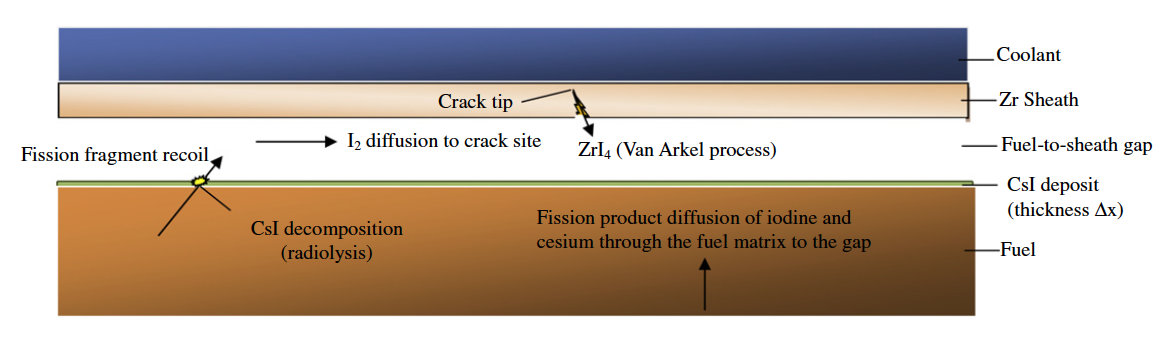
\includegraphics[width=\linewidth]{images/vanarkel.png}
\caption[Schematic of a proposed I-SCC process for cladding crack penetration.]{Schematic of a proposed I-SCC process for cladding crack penetration. Taken from \cite{Lewis2011}.}
\label{figure:vanarkel}
\end{figure}


\subsection{Iodine availability}

The amount of free iodine available in the fuel pin is dependent on many different factors (e.g. temperature, pressure, power history, axial location in fuel pin, diffusion rate through fuel), making it difficult to measure. Additionally, iodine nuclei (and fission products in general) will likely implant in either the fuel pellet or the cladding due to their large kinetic energies following a fission event. 

\subsubsection{Radiolysis}

Thermodynamic calculations performed by Konashi \emph{et al}. estimate the equilibrium partial pressure of iodine in the fuel-cladding gap to be as low as 10$^{-17}$ atm when there is no radiolysis of CsI, and up to 10$^{-8}$ atm with the effect of CsI radiolysis included \cite{Konashi1983}. For comparison, mandrel tests of irradiated Zr claddings at 350 $^{\circ}$C show that susceptibility to I-SCC is reduced when the iodine partial pressure is below 60 Pa (approximately 6$\times 10^{-4}$ atm) \cite{anghel2010experimental}. While these calculated values of the iodine pressure are too low to induce corrosion in Zr, they demonstrate that radiation will increase the partial pressure of iodine by several orders of magnitude. Increasing reactor power (e.g. during a ramp) will increase radiation flux and therefore dissociation of CsI, however, no figures are yet available which demonstrate a clear link between this contribution to the iodine pressure and PCI failures. 

\subsubsection{Implantation}

Fission products immediately following a fission event have kinetic energies of up to 90 MeV. These are large, highly ionising particles which deposit their energy to the surrounding atoms within several microns of where they are produced, due to the large electronic and nuclear stopping power of crystalline solids such as UO$_{2}$ and ZrO$_{2}$. Figure \ref{figure:srimtrim}a shows TRIM calculations of the amount of iodine that is implanted in ZrO$_{2}$ at different incident ion energy levels. 

\begin{figure}[ht] % SRIM/TRIM values for iodine in ZrO2
\centering
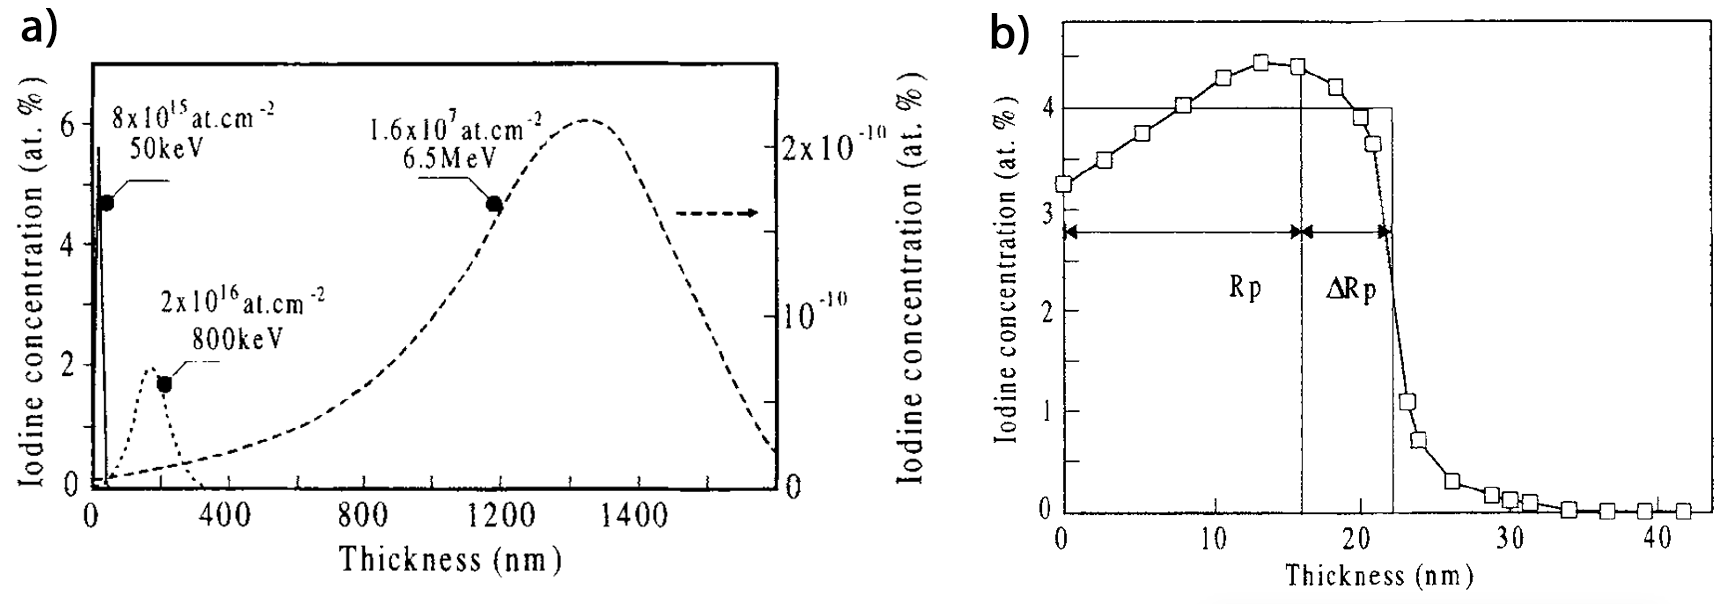
\includegraphics[width=\linewidth]{images/srimtrim.png}
\caption[\textbf{a)} TRIM distributions for iodine implantation in ZrO$_{2}$ at 50 keV, 800 keV and 6.5 MeV. \textbf{b)} Rutherford backscattering spectrometry profile of 50 keV iodine implanted in ZrO$_{2}$ samples.]{\textbf{a)} TRIM distributions for iodine implantation in ZrO$_{2}$ at 50 keV, 800 keV and 6.5 MeV. \textbf{b)} Rutherford backscattering spectrometry profile of 50 keV iodine implanted in ZrO$_{2}$ samples. Taken from \cite{brossard1998use}.}
\label{figure:srimtrim}
\end{figure}

Further to the mechanism described above, it is important to consider the role of oxygen in the I-SCC process. Fuel pins do not regularly fail during normal operation, despite iodine being produced continuously from fission of the fuel. As previously mentioned, this is because the inner surface of the cladding is not pure Zr metal, but rather a protective oxide which provides an effective barrier against corrosive species such as iodine.

\section{Oxidation of zirconium}

The oxidation of zirconium to produce \zirconia\ occurs during manufacture of the fuel cladding when the Zr metal is exposed to oxygen in air. \zirconia\ is a ceramic with material properties that make it desirable in many industrial applications, including solid-oxide fuel cells \cite{radford1979zirconia}, refractory linings \cite{whittemore1952fused}, and nuclear waste storage \cite{wang2012ceramics}. However, in the context of nuclear fuel cladding, the most important function of \zirconia\ is the barrier it provides against the ingress of corrosive species. 

\zirconia\ grown thermally on Zr metal exists mainly in either the monoclinic or tetragonal phase \cite{Howard1988,teufer1962crystal}. We can expect the internal \zirconia\ layer of the cladding to be mostly monoclinic in early life, with the stress-stabilised tetragonal phase appearing near the oxide/metal interface due to cohesive strains resulting from the lattice mismatch. With increasing burnup, it is expected that more tetragonal and possibly even the cubic phase of \zirconia\ forms due to anion vacancy formation and residual stresses in the lattice from radiation damage \cite{sickafus1999radiation}. Amorphisation due to radiation damage has also been observed in the cubic phase from Cs$^{+}$ implantation \cite{amorphization2000wang}. In this thesis however, while defect energies for the cubic phase are reported (see Figures \ref{isolated_defects}, \ref{table:bound_defects}, \ref{figure:cubicinter}), the focus is on monoclinic and tetragonal \zirconia\ phases, partly due to difficulties predicting the behaviour of the pure high-temperature cubic phase using energies calculated from a static energy technique. 

\subsection{Oxide growth mechanism}

An oxide layer will form on the surface of zirconium metal even at very low oxygen partial pressures \cite{causey2005review}. The oxidation process is mainly driven by the ingress of oxygen ions. Initially, the oxide is highly protective, growing slowly into the metal until it reaches a thickness of approximately 2-3 $\mu$m \cite{garzarolli1991oxide, dawson1968kinetics}, after which the oxide growth mechanism enters a `post-transition' stage where the oxidation kinetics follow a cubic-rate law  \cite{porte1960oxidation}. At low temperatures relative to the melting point or high pressures, and after reaching a critical thickness (called the transition point), parts of the initial oxide will fail and the oxidation rate will increase again. This process is illustrated in Figure \ref{figure:oxide_weight_gain}. 

\begin{figure}[ht]
\centering
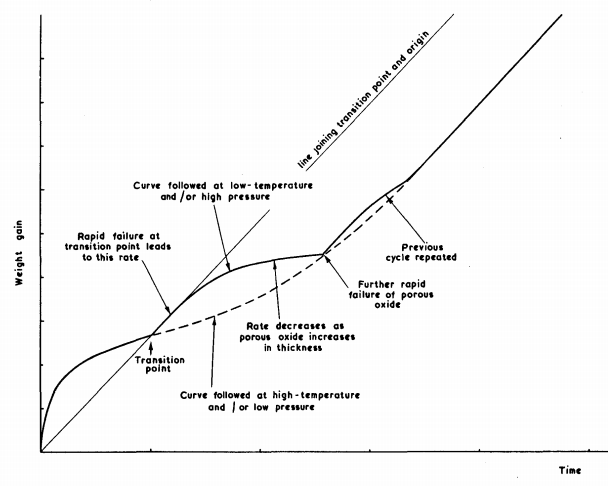
\includegraphics[height=10.5cm]{images/zro2_oxide_weight_gain.png}
\caption[Diagrammatic representation of the cyclical oxidation behaviour of \zirconia .]{Diagrammatic representation of the cyclical oxidation behaviour of \zirconia . Taken from \cite{cox1963some}.}
\label{figure:oxide_weight_gain}
\end{figure}

\subsection{Oxygen solubility of zirconium}

Considering the Zr-O binary phase diagram in Figure \ref{figure:binary_phase_diagram}, oxygen is soluble in zirconium up to 29\% of total molar mass when below 400 $^{\circ}$C, commensurate with the operating temperature of a typical PWR (330 \textdegree C at the outer surface of the cladding). Solubility increases slightly up to 35\% of total molar mass as temperature is increased to the liquidus line at 2065 $^{\circ}$C. This is important to note because in the literature, it is assumed that there is pure Zr metal immediately beneath the \zirconia\ layer \cite{rossi2015first}, which is an assumption that will underestimate the extent to which repassivation occurs when the oxide layer is breached, and disregards the effect of the thin ZrO interface that can precede the metal. The molar mass of oxygen required to grow more oxide near the interface will therefore be at least 37\% lower than expected when using this assumption.

The presence of oxygen in the Zr metal will also have an effect on thermodynamic calculations of extrinsic defect formation. Atoms such as Te and I will have to compete with O atoms (and potentially, self-interstitial Zr atoms) for interstitial sites in the metal. This increases the energy barrier to diffusion because of the lower availability of sites. An energy input is required to remove O or Zr atoms occupying these sites, making them a less favourable diffusion path.


\begin{figure}[ht]
\centering
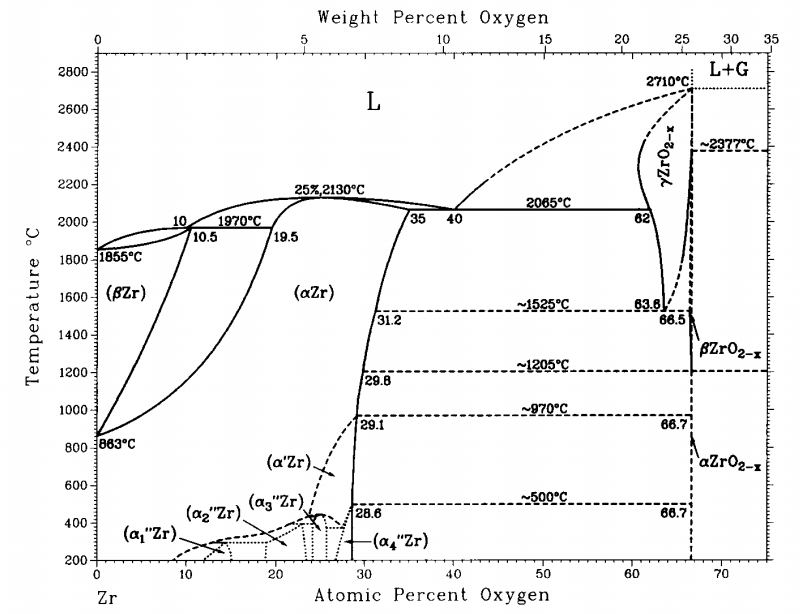
\includegraphics[width=14cm]{images/zro2_binary_phase.png}
\caption[Binary phase diagram of the Zr and O$_{2}$ system.]{Binary phase diagram of the Zr and O$_{2}$ system. Taken from \cite{Abriata1986}.}
\label{figure:binary_phase_diagram}
\end{figure}

\subsection{Outer oxide vs inner oxide} \label{section:outervsinner}

As mentioned previously, the cladding of an LWR fuel pin develops an oxide on both the inner and outer surfaces due to exposure to oxygen in air during manufacture. Both the outer and inner oxide layers provide protection against corrosion, though the corrosive environment is different. 

The outer oxide layer is in contact with the coolant, which is mostly light water with some additional dissolved species such as boron and hydrogen to control reactivity and pH. Figure \ref{figure:outer_oxide} shows a section of the cladding with the outer oxide visible. This layer is mostly monoclinic \zirconia\ with small (nano) grains of tetragonal \zirconia\ distributed uniformly throughout. These grains of tetragonal \zirconia\ are autostabilised during growth of the oxide because of the large volume expansion associated with oxidation (Zr has a Pilling-Bedworth ratio of 1.57). Of course, transmission electron microscope (TEM) foils under examination are always stress-relieved, whereas the oxide in reactor conditions will be under 1-2 GPa of residual stress due to the growth of the oxide (see § \ref{section:tet_stress_stabilisation}).

\begin{figure}[ht]
\centering
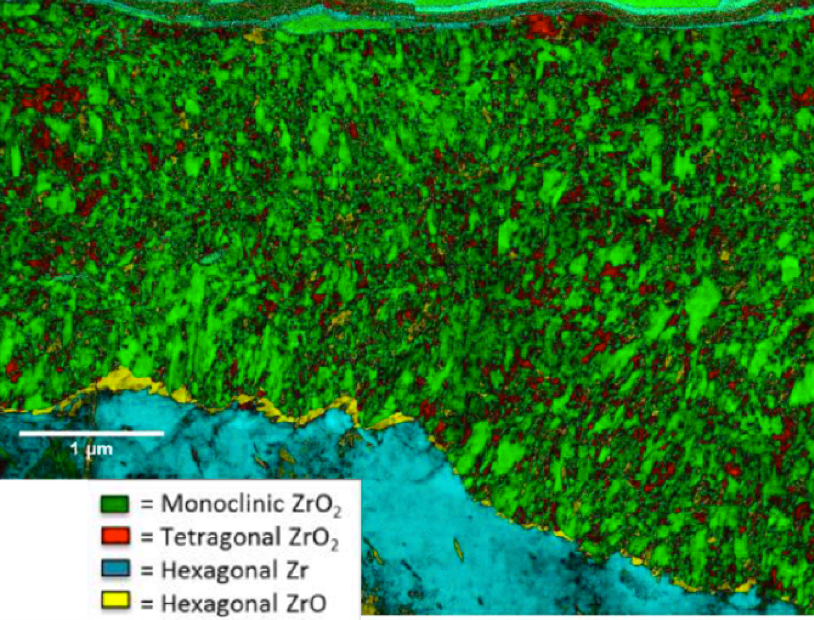
\includegraphics[height=10.5cm]{images/outer_oxide.png}
\caption[Scanning transmission electron microscrope (STEM) image of the outer oxide layer formed in an autoclave under simulated PWR water conditions showing the prevalence of different \zirconia\ phases.]{Scanning transmission electron microscrope (STEM) image of the outer oxide layer formed in an autoclave under simulated PWR water conditions showing the prevalence of different \zirconia\ phases. Taken from \cite{Hu2016}.}
\label{figure:outer_oxide}
\end{figure}

The internal oxide layer is much more challenging to examine due to the need to prepare samples in hot cells. This layer is typically very brittle due to radiation damage and implantation of fission products. At a high enough burnup, the \zirconia\ layer makes contact with the UO$_{2}$ fuel, with which it will bond. Figure \ref{figure:inner_oxide} shows a section of the cladding with the inner oxide layer bonded to the pellet. The crystal structure of the \zirconia\ in this layer is debated. Some studies report no monoclinic phase in high burnup fuels, with cubic phase \zirconia\ throughout most of the layer and an amorphous phase nearer the pellet side \cite{Nogita1997}, while other studies report mostly tetragonal phase in this layer \cite{ciszak2017etude, gibert1998influence}. 
%After removal from the reactor and the subsequent cooling period, the inner oxide

\begin{figure}[ht]
\centering
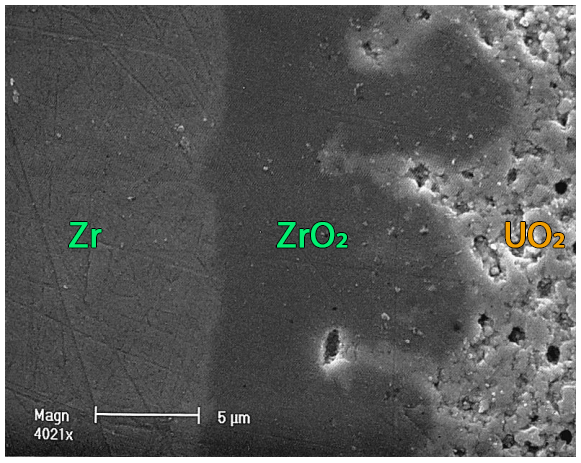
\includegraphics[height=10.5cm]{images/pci_bondinglayer.png}
\caption[High resolution scanning electron microscrope (SEM) image of the bonding layer between a PWR UO$_{2}$ fuel pellet and Zr cladding in a fuel pin at an approximate burnup of 60 GWd/tU.]{High resolution SEM image of the bonding layer between a PWR UO$_{2}$ fuel pellet and Zr cladding in a fuel pin at an approximate burnup of 60 GWd/tU. Adapted from \cite{Lozano1998}.}
\label{figure:inner_oxide}
\end{figure}

Figure \ref{figure:bonding_layer_composition} shows the composition of the inner oxide of a high burnup fuel pin. The fission product (Ba, Mo, Nd) content is highest at the beginning of the \zirconia\ layer and decreases almost linearly with distance towards the Zr metal. This is due to fission product implantation rather than diffusion in the oxide as these elements have low volatility and low cation diffusion rates in UO$_{2}$ where they are produced \cite{S.G.PrussinD.R.OlanderP.Goubeault1984, Prussin1988}. % can you use the weight composition and fission yields to estimate what percentage of iodine implantation will be?

\begin{figure}[ht!]
\centering
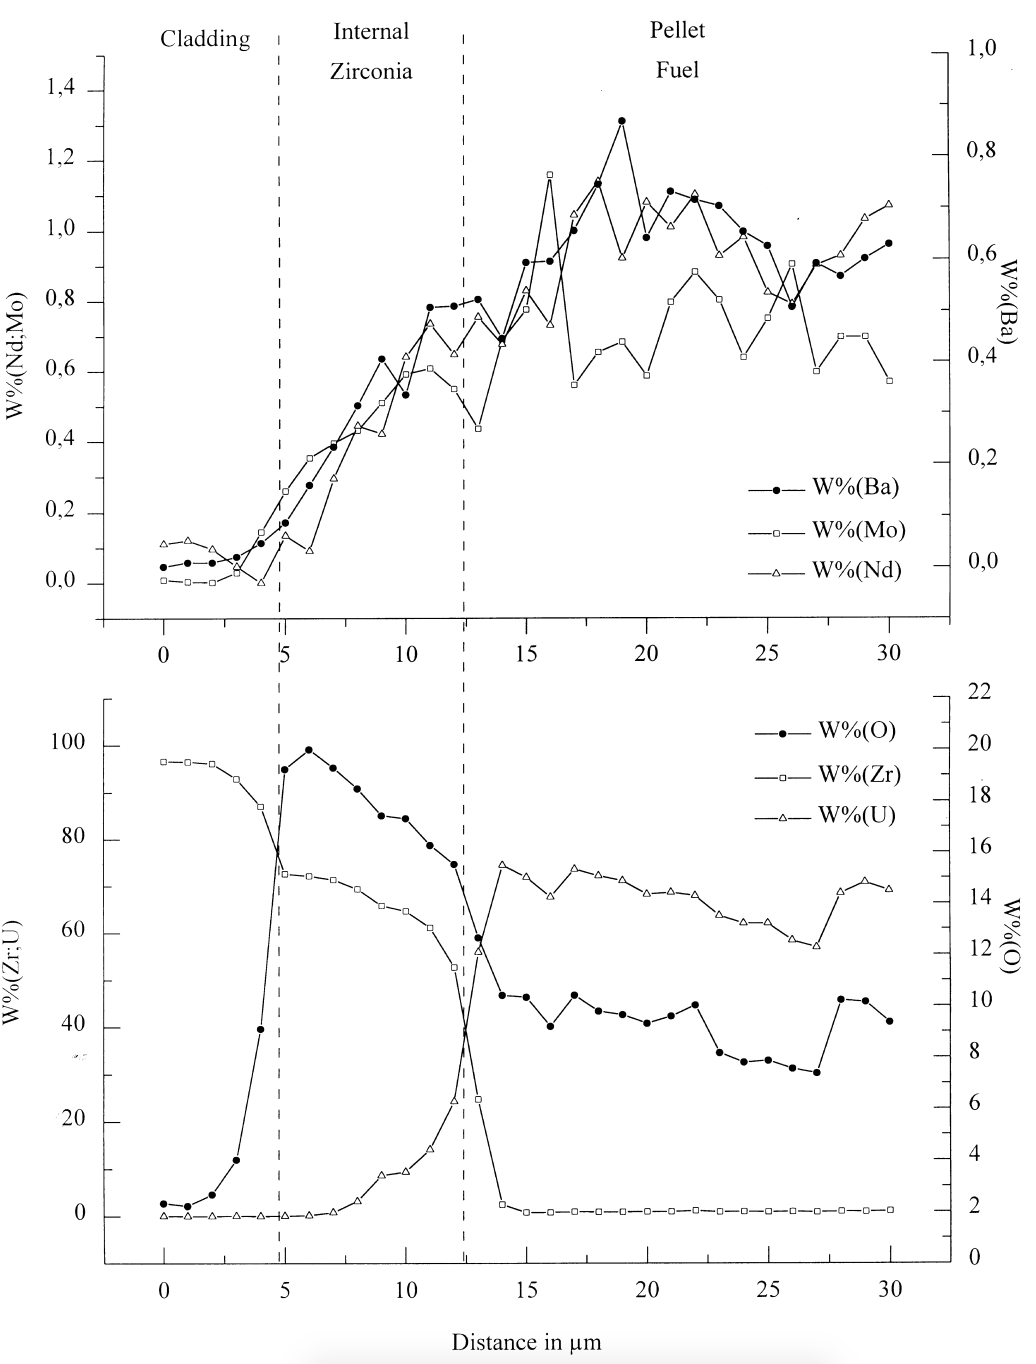
\includegraphics[width=14cm]{images/bonding_layer_composition.png}
\caption[Elemental composition of the bonded UO$_{2}$/ZrO$_{2}$ layer from a PWR UO$_{2}$ fuel pellet with a burnup of 61 GWd/tU.]{Elemental composition of the bonded UO$_{2}$/ZrO$_{2}$ layer from a PWR UO$_{2}$ fuel pellet with a burnup of 61 GWd/tU. Taken from \cite{Lozano1998}.}
\label{figure:bonding_layer_composition}
\end{figure}


\subsection{Sources of oxygen}

The internal oxide layer is present before fuel claddings are pressurised with helium gas and sealed. This is from the normal oxidation of Zr in air, where the oxygen pressure is 0.21 atm. After capping of the fuel rods, the only other available oxygen is from the UO$_{2}$ fuel pellets.

Uranium oxides have a wide range of non-stoichiometric compositions, with U/O ratios ranging from 1.67 to 2.24 in solid UO$_{2 \pm x}$, as shown in Figure \ref{figure:U_O_phase_diagram}. The oxide form U$_{3}$O$_{8-y}$ also exists and is more kinetically and thermodynamically stable than UO$_{2}$, but has lower density, making it less suitable for use as a fuel form. The different stoichiometries have different equilibrium O$_{2}$ pressures at constant temperature, allowing some level of internal cladding environment control depending on whether more or less oxygen is desired. 

Oxygen and oxygen precursors may also be produced directly from fission of U$_{235}$, but this contribution is insignificant compared to changing the stoichiometry of the fuel pellet. That is, liberation of oxygen from UO$_{2 \pm x}$ due to fission (which is also a function of the fuel's stoichiometry) is a more significant contributor to the oxygen pressure than direct production via fission.

\begin{figure}[ht!]
\centering
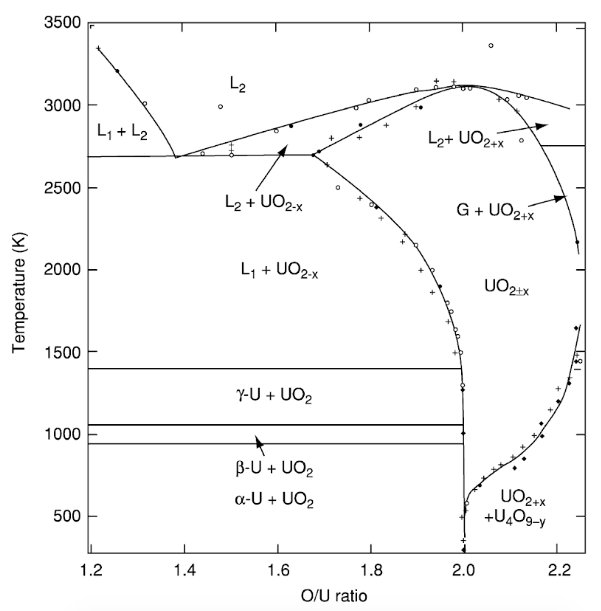
\includegraphics[height=12cm]{images/UO_phase_diagram.png}
\caption[Partial U-O temperature phase diagram between O/U ratios of 1.2 and 2.25.]{Partial U-O temperature phase diagram between O/U ratios of 1.2 and 2.25. Figure taken from \cite{katz2007chemistry}, with phase boundaries from \cite{rand1978thermodynamic, chevalier2002progress, gueneau2002thermodynamic}.}
\label{figure:U_O_phase_diagram}
\end{figure}


\section{Atomistic Simulation}

Conducting experiments on active nuclear materials is a difficult undertaking. Handling irradiated materials is an expensive process, and materials such as uranium are highly controlled (though they are relatively benign before irradiation compared to many typical chemical laboratory materials and solvents). Furthermore, experiments which require samples to be irradiated must be left to cool-down (due to material activation) for up to a year before they can be analysed in a specialised lab \cite{efthymiopoulos2011hiradmat}. Thus, any errors in the experimental procedure or problems with samples are not revealed until months later when material analysis is performed. This makes it difficult to study many material phenomena, especially if they are time-dependent. In-situ reactor experiments are also problematic, requiring sensor equipment to be made tolerant to the high radiation environments as well as being acceptable to and consistent with the reactor operation safety case. The risks and costs mean that experimental work is mostly restricted to the largest labs and the few researchers with enough funding to support it.

\subsection{Classical approach - molecular dynamics}

Molecular dynamics (MD) uses classical mechanics as the basis for calculations. These types of simulations typically use pair potentials (though many-bodied potentials are also used). These are mathematical functions which effectively describe the energy of interaction between two particles. Pair potentials are created by fitting functions to several parameters from empirical data, such as equilibrium bond lengths, thermal properties or even values from quantum mechanical calculations. The simple form of pair potentials allows MD simulations to scale up to billions of atoms, corresponding to a length scale of approximately 0.1 $\mu$m. 

In the literature, many molecular dynamics studies of \zirconia\ exist. However, these studies typically focus on dopant-stabilised zirconias (i.e. cubic ones as empirical potentials don't capture monoclinic or tetragonal phases and their transitions accurately). The large system sizes possible in molecular dynamics simulations are often necessary for examining properties such as ion diffusion, thermal conductivity or melting points \cite{Davis2010}. Studying fission products in \zirconia\ however, requires potentials which can accurately model interactions of atoms such as Zr, O, and I in the solid phase. A good potential for such a system has not yet been published and so a quantum mechanical study of the \zirconia\ system is the focus of this thesis. The work herein may then be used in the future development of such potentials.

%These relatively large system sizes make MD a useful tool for studying a range of materials phenomena which are difficult to model at smaller scales, such as dislocations and long-range diffusion. 

%Add a figure here showing lennard jones. Also show the basic equations
%These are mainly pair potentials (although many-bodied potentials are also used) which are some combination of a short-range repulsion term (Pauli exclusion, nuclear repulsion if van der waals is taken into account) and a long range Coulombic attraction term

\subsection{Quantum mechanical approach - DFT}

Another method for modelling materials at the atomic scale is to use a quantum mechanical approach. In this thesis, the framework of density functional theory (DFT) is used throughout for quantum mechanical calculations (see § \ref{section:dft}). These techniques use a more fundamental approach than molecular dynamics, and are sometimes referred to as \emph{ab initio} methods (although several empirical approximations are often used in DFT). The CASTEP 8.0 software package was used for all DFT calculations \cite{Clark2005}.

System sizes are far more constrained when using DFT. The equations being solved scale combinatorially with the number of electrons and ions in the system, quickly becoming intractable even for simple molecules with a few atoms before applying DFT methods. There are several ways to significantly reduce the computational complexity without sacrificing too much accuracy (e.g. the pseudopotential method, periodic boundaries, cell constraints and symmetry). This allows system sizes on the order of hundreds of atoms to be studied, corresponding to a length scale of approximately 1 nm. While this length scale is much smaller than what can be achieved using MD, the use of a more fundamental parameter (electron density) in calculations provides a stronger scientific basis when material properties are derived from DFT models. Additionally, DFT allows electronic properties such as electron orbital occupancy and band gaps to be studied.

In the literature, DFT studies of \zirconia\ are predominantly focused on the dopant-stabilised cubic phase because of its use in fuel cells and medical applications \cite{orera1990intrinsic,jiang2011first}, with few studies on the undoped system \cite{mackrodt1986theoretical,aarhammar2009energetics}. Pure oxide studies also tend to focus on only one of the three common phase, typically the monoclinic \cite{zheng2007first,foster2002modelling,foster2001structure} and tetragonal phases \cite{Gionco2013, Eichler2004, Zhang2014}. Two notable studies have looked at all three phases. The first focused on the electronic structure and optical properties of \zirconia\ \cite{French1994}, while the second examined the structural properties and band structure of \zirconia\ \cite{Kralik1998}. Both studies utilised the LDA exchange-correlation functional. This functional has since been improved upon (see § \ref{section:kohnsham}), improving the accuracy of more recent models. However, it is always useful to compare to data from older studies. 

Lattice dielectric properties in the three phases have been calculated using DFT \cite{Zhao2002a}, and these have been used in this thesis to predict energies and defect equilibria. Various data from these studies have been used either for comparison or to aid in new calculations which have then been published.

\subsection{Band gap}

Conductors and insulators are two common ways to describe materials. While this binary characterisation may work as an approximation for many materials, in reality there is more of a continuum between these two states (e.g. semiconductors), and at the heart of this lies the band gap.

It is known that for ions, electron energy levels are quantised, restricting the range of possible electron energies to discrete quantities. More specifically, electrons can only occupy unique quantum states, defined by parameters such as quantum spin and angular momentum. In a crystal, where there are large numbers of electrons and many possible configurations of them, we refer to energy \emph{bands} which are comprised of many quantised energies. There are sometimes gaps between energy bands in crystals (illustrated in Figure \ref{figure:band_gap}) corresponding to energy levels that cannot be occupied, meaning that if electrons were to be added at the lowest energy levels one by one, there would occasionally be relatively large jumps in energy as an electron is forced to enter a higher energy band. 

\begin{figure}[ht]
\centering
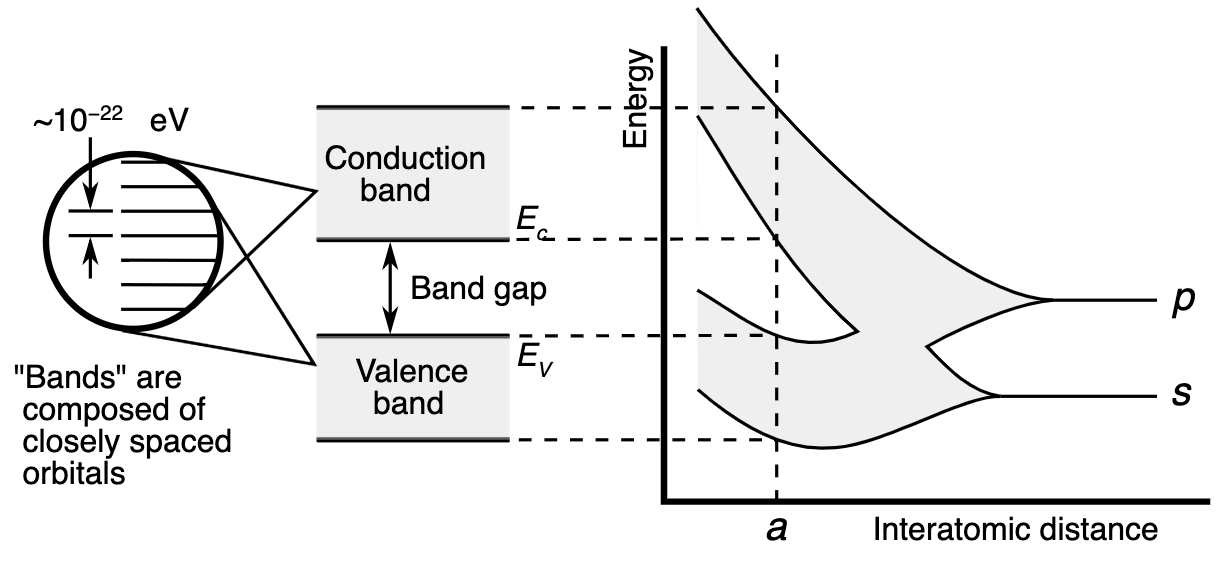
\includegraphics[width=\linewidth]{images/band_gap.png}
\caption[Illustration of the band gap in diamond as a function of interatomic spacing.]{Illustration of the band gap in diamond as a function of interatomic spacing. Taken from \cite{Chetvorno2017}.}
\label{figure:band_gap}
\end{figure}

Two energy bands, the \emph{valence band} and \emph{conduction band}, help determine a material's metallic or non-metallic character. The valence band contains energy levels occupied by the valence electrons (at absolute zero), while the conduction band contains energy levels which are high enough that electrons may freely move throughout the crystal. In metals, the valence and conduction bands have some amount of overlap, meaning that once the valence band is full, the highest occupied electron energy states are within the conduction band and so the material acts as a conductor. Materials like \zirconia , however, have large energy gaps between the valence and conduction bands, known as the band gap. These materials are called \emph{band insulators} (as opposed to \emph{Mott insulators} where there is no conventional band gap, but electron-electron interactions impede electron promotion to higher energies), because the band gap is an energy barrier preventing the valence electrons from moving freely around the crystal. 

In addition to the valence and conduction bands, a value for the electron chemical potential or Fermi level of the material is needed to determine how the energy bands are filled. If the Fermi level is exactly halfway between the valence band maximum (VBM) and the conduction band minimum (CBM), then the additional energy input required to promote an electron to the conduction band is half of the band gap. The Fermi level is strongly dependent on extrinsic defects and temperature. Extrinsic defects (called dopants) can be introduced to materials such as semiconductors in order to change the concentration of electronic defects (electrons and holes), while an increase in temperature will result in an increase in the Fermi level because of the larger quantity of thermal energy available.

It is important to note that band gaps reported in DFT studies using classical LDA/GGA methods are significantly lower than those obtained experimentally. This is a known problem in DFT, and an exchange-correlation functional which reproduces correct band gap energies in semiconductors and insulators (without overfitting to experimental data) has not yet been discovered. The GW method, which uses a self-energy energy term in place of an exchange-correlation functional, allows more accurate\footnote{The GW approximation still has inaccuracies when modelling strongly correlated systems, but works well with $s$-$p$ systems.} estimates of the band gap than with DFT, but at a significantly higher computational expense. In many cases, the band gap from DFT calculations may be increased by appending an additional potential term, known as a +U parameter, to certain valence electron orbitals (discussed further in § \ref{subsection:plus_U}), or by using hybrid potentials which can incorporate the exact exchange energy.








%\section{Fission product empirical potential}
%
%In order to study the interaction of fission products with larger features in the cladding microstructure, such as dislocations and grain boundaries, it is necessary to develop empirical potentials for use in molecular dynamics simulations. Grain boundary transport is of particular interest, and this would require something on the order of 10$^{4}$ atoms to simulate to a reasonable degree of accuracy. This cannot be done using DFT currently due to the significant amount of computing resources required to run such a simulation. 
%
%The development of an iodine and xenon potential with \zirconia\ should be prioritised in order to run simulations to determine the migration of iodine within \zirconia, followed by the behaviour of xenon at the equilibrium iodine sites.
%
%\section{Grain boundary transport}
%
%Grain boundaries are interesting areas for studying species migration because diffusion towards the metal is expected to be more rapid through them than through bulk \zirconia .
%
%\section{Zr/ZrO/\zirconia\ interface study}
%
%The inner oxide is not a homogeneous structure, as described in § \ref{ch:crystallography}. Figure \ref{fig:zro_interface} clearly shows the existence of a ZrO phase up to 200 nm thick at the interface between \zirconia\ and Zr metal. The presence of ZrO and even oxygen-saturated Zr metal will have an effect on the thermodynamic equilibria of different fission products. An interface study can be conducted using DFT, to determine stresses at the interfaces of Zr and ZrO, and ZrO and \zirconia . Studying the aggregate effect of these interfaces on fission product behaviour may require larger molecular dynamics simulations, however. The crystal structure of the ZrO phase has been studied using both simulation and high-resolution electron microscopy, with two likely crystal structures being proposed \cite{Nicholls2015}. Further atomistic studies must be conducted to determine the stability of each crystal structure of ZrO when constrained by \zirconia\ and oxygen-saturated Zr metal interfaces.
%
%
%\begin{figure}[ht]
%    \centering
%    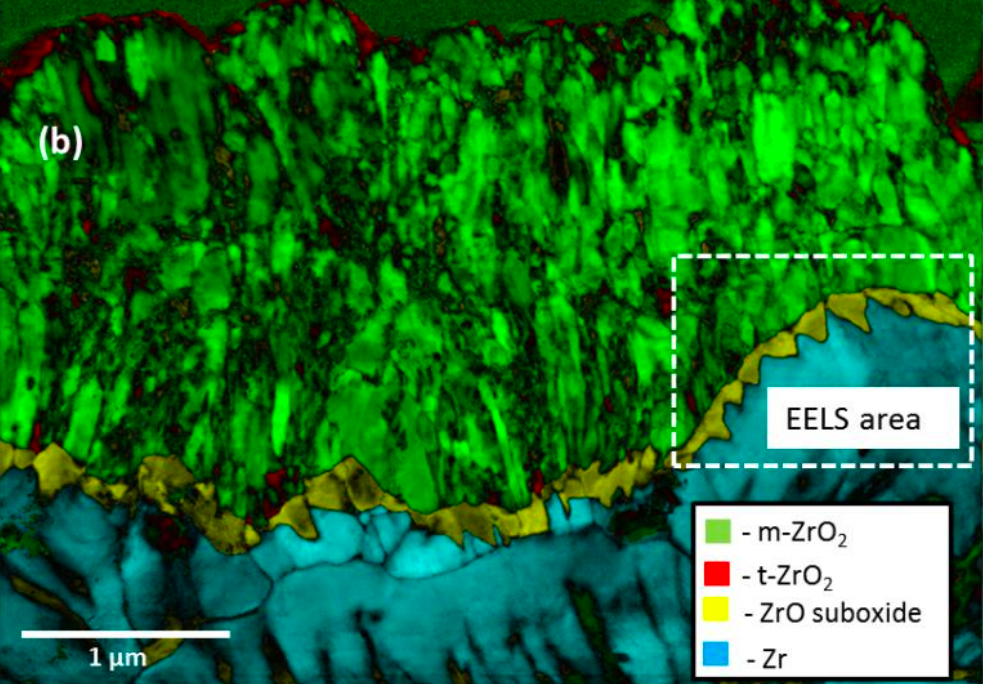
\includegraphics[height=9cm]{images/zro_interface.png}
%    \caption[STEM image of a Zr-1.0\%Nb sample oxidised in simulated PWR water at 360 C for 120 days.]{STEM image of a Zr-1.0\%Nb sample oxidised in simulated PWR water at 360 C for 120 days. Taken from \cite{inproceedings}.}
%    \label{fig:zro_interface}
%\end{figure}